\documentclass[12pt]{article}
\author{Lawrence Liu}
\usepackage{subcaption}
\usepackage{graphicx}
\usepackage{amsmath}
\usepackage{pdfpages}
\newcommand{\Laplace}{\mathscr{L}}
\setlength{\parskip}{\baselineskip}%
\setlength{\parindent}{0pt}%
\usepackage{xcolor}
\usepackage{listings}
\definecolor{backcolour}{rgb}{0.95,0.95,0.92}
\usepackage{amssymb}
\lstdefinestyle{mystyle}{
    backgroundcolor=\color{backcolour}}
\lstset{style=mystyle}

\title{ECE 231A HW 3}
\begin{document}
\maketitle
\section*{Problem 1}
\subsection*{(a)}
\begin{align*}
    \lim_{n\to\infty}[p(X_1,\cdots,X_n)]^{\frac{1}{n}}&=
        2^{\lim_{n\to\infty}\frac{1}{n}\log_2[p(X_1,\cdots,X_n)]}\\
    &=2^{\lim_{n\to\infty}\frac{1}{n}\sum_{i=1}^n\log_2[p(X_i)]}\\
    &=2^{E[\ln[p(X_i)]]}\\
    &=\boxed{2^{H(x)}}
\end{align*}
\subsection*{(b)}
\begin{align*}
    E\left[\left(\prod_{i=1}^nf(X_i)\right)^{\frac{1}{n}}\right]&=
        \exp\left[\ln\left(E\left[\left(\prod_{i=1}^nf(X_i)\right)\right]\right)\right]\\
    &\leq \exp\left[\frac{1}{n}E\left[\ln\left(\prod_{i=1}^nf(X_i)\right)\right]\right]\\
    &=\exp\left[\frac{1}{n}\sum_{i=1}^nE\left[\ln\left(f(X_i)\right)\right]\right]\\
    &\leq \exp\left[\frac{1}{n}\sum_{i=1}^nE[X_i]\right]\\
    &=\exp\left[E[X_i]\right]
\end{align*}
Therefore we have that
$$
    \boxed{E\left[\left(\prod_{i=1}^nf(X_i)\right)^{\frac{1}{n}}\right]\leq \exp\left[E[X_i]\right]}
    $$
\section*{Problem 2}
\subsection*{(a)}
$$H(X)=\boxed{1.895}$$
\subsection*{(b)}
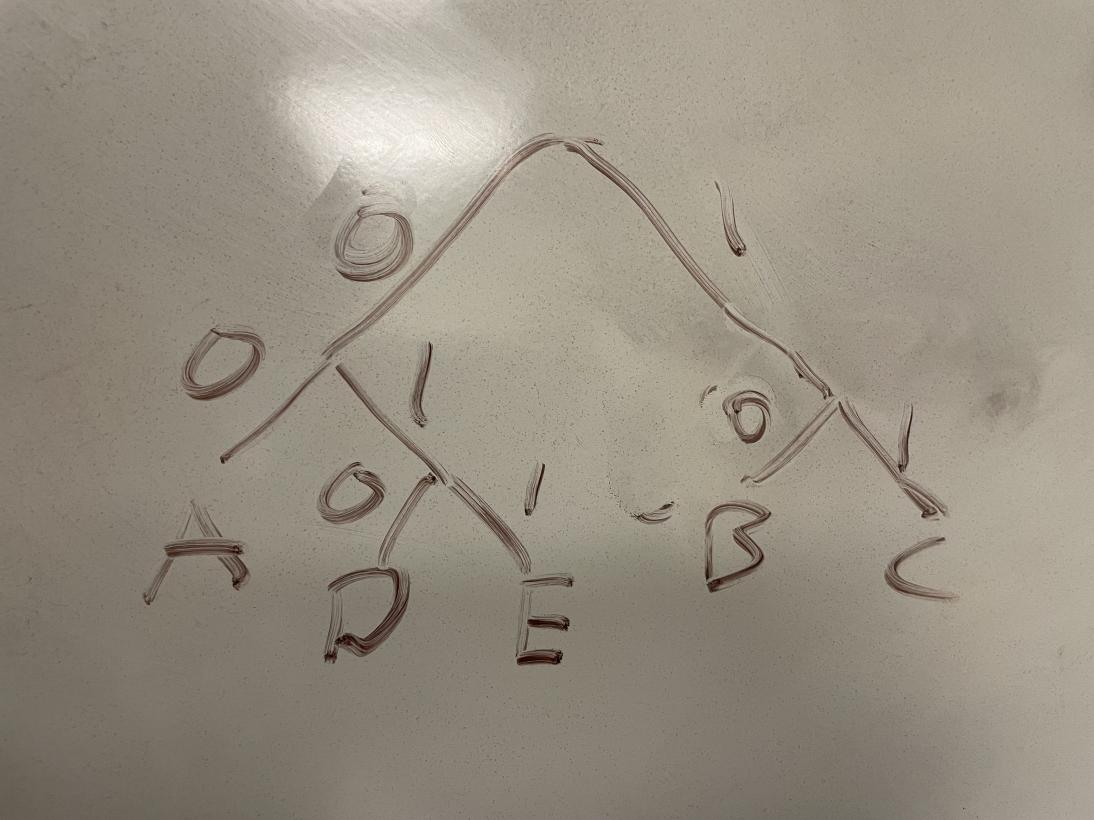
\includegraphics[scale=0.25]{fig1.jpg}\\
So we have that the average length is $\boxed{2.3}$ bits.
\subsection*{(c)}
codeword A is 001\\
codeword B is 0011\\
codeword C is 0101\\
codeword D is 1101\\
codeword E is 10011\\
Therefore the SFE codeword average length is $\boxed{3.8} bits$.
\subsection*{(d)}

\end{document}